\subsection{Strukturierung der Evaluation der Architektur}
\label{sec:methodik-evaluation}

Damit über die Einordnung der Traceability-Architektur selbst und den Varianten der Traceabilityarchitektur aus \fullref{sec:traceability-architecture} eine Aussage ob einer optimalen Architektur (im Sinne der leitenden Fragestellung) gemacht werden kann ist folgende Methodik vorgesehen:

\begin{enumerate}
    \item Identifikation relevanter Bewertungsdimensionen für die Architektur selbst wie die Varianten
    \item Recherche und Ableitung von Kriterien innerhalb der Bewertungsdimensionen (sowohl vom \ac{bit} als auch aus der Literatur)
    \item Ableitung eines Konformitätschecks der Traceability-Architektur an sich
    \item Ableitung Bewertungsprozesses für die Traceability-Architektur Varianten
    
\end{enumerate}

Basierend auf der Orientierung an \ac{togaf} wird sich bei der Suche an Dimensionen an dem \ac{adm} Cycle orientiert. Folgende Dimensionen werden ausgewählt:

\begin{longtable}{|
  L{3cm}|
  p{\dimexpr(\textwidth-3cm-6\tabcolsep-4\arrayrulewidth)/2\relax}|
  p{\dimexpr(\textwidth-3cm-6\tabcolsep-4\arrayrulewidth)/2\relax}|
}
    \hline
    \textbf{Dimension} & \textbf{Beschreibung} & \textbf{Begründung} \\
    \hline
    \endfirsthead

    \hline
    \textbf{Dimension} & \textbf{Beschreibung} & \textbf{Begründung} \\
    \hline
    \endhead

    Architekturprinzipien &
    Prinzipien oder grundlegende Eigenschaften einer Architektur. Architekturprinzipien können eingehalten oder nicht eingehalten sein. Dies ist eine Evaluationsdimension, welche auf die Traceability-Architektur als angewendet wird &
    Ergeben sich aus der Preliminary Phase im \ac{adm} Cycle in welcher die allg. Rahmenbedingungen gesetzt werden, von der Architekturprinzipien teil sind. Die Architekturprinzipien sind als Gatekeeper für Varianten gedacht
    \\
    \hline
    Qualitätsmerkmale &
    Qualitative Eigenschaften der Architektur analog zu klassischen \ac{nfr}. Qualitätsmerkmale können basierend auf einer Skala zu einem gewissen Mass erfüllt sein. Dies ist eine Evaluationsdimension, welche auf die verschiedenen Varianten der Architektur angewendet wird &
    Ergeben sich gedanklich aus den Phasen A-D im \ac{adm} Cycle und dienen als vergleichende Kriterien zwischen verschiedenen Varianten
    \\
    \hline
    Entscheidung und Trade-Off &
    Spannungsfelder unterschiedlicher Architekturrichtungen welche nicht per se richtig oder falsch sind. Trade-Off Kriterien werden zum Labeling / zur Charakterisierung verwendet. Dies ist eine Evaluationsdimension, welche auf die verschiedenen Varianten der Architektur angewendet wird &
    Ergibt sich gedanklich aus den Phasen E-F im \ac{adm} Cycle. Sollen die Eigenschaften der unterschiedlichen Varianten hervorheben, ohne wertend zu wirken, da die durch das Kriterium vergleichenden Eigenschaften  grundsätzlich keine negative/positive Konnotation besitzen sollen
    \\
    \hline
    Kontext und Anwendung &
    Konkrete Rahmenbedingungen aus dem \ac{bit} Use-Case, welche den Bewertungskontext der Evaluationskriterien bzw. Evaluationsdimensionen beeinflusst. &
    Ergibt sich aus der Festlegung des Kontextes in der Preliminary Phase und Ausarbeitung in den Phasen B-D im \ac{adm} Cycle. Dient dazu im Rahmen des definierten Use-Cases zu beurteilen. Im Gegensatz zu den Architekturprinzipien des \ac{bit} ist der Use-Case flexibler
    \\
    \hline
    \caption{Identifizierte Dimensionen des Evaluationsframeworks}
    \label{tab:evaluation-dimensions}
\end{longtable}

Die Architekturprinzipien vom ac{bit} bilden sich aus den Vorgaben, welche durch die Organisation selbst vorgegeben sind. Von weiteren Kriterien vom \ac{bit} für die Arbeit wird abgesehen. Die Architekturprinzipien aus \autoref{fig:bit-architecture-principles} gelten für das gesamte \ac{bit}.

\begin{figure}[H]
    \centering
    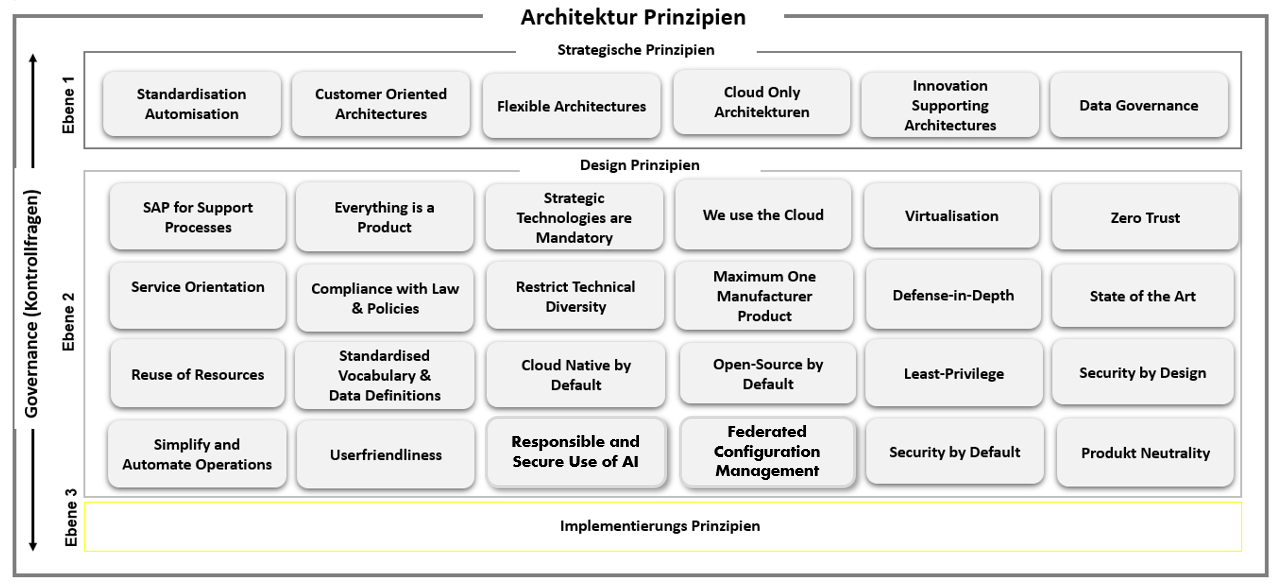
\includegraphics[width=\textwidth]{graphics/bit-architektur-prinzipien.png}
    \caption{Architekturprinzipien des \ac{bit} \parencite{noauthor_vorgabenportal_2025}}
    \label{fig:bit-architecture-principles}
\end{figure}

Für diese Arbeit werden die Prinzipien je nach gewähltem Use-Case selektiv berücksichtigt. Zu den Kriterien des \ac{bit} sollen weitere identifiziert werden, welche explizit für den Umstand der multi-Cloud ready \ac{ea} vorgesehen sind. Hierfür werden initial die folgenden Recherchefragen formuliert:

\flqq What are possible architecture princples for multi-Cloud ready enterprise architectures and solution architectures?\frqq\hspace{0.05cm}, welche mit Elicit AI recherchiert wurde (siehe Tools in \fullref{sec:hilfsmittel}). Die identifizierten Prinzipien zeigen, dass die Frage mit dem Begriff \flqq solution architecture\frqq\hspace{0.05cm} bereits zu stark auf konkrete technische Prinzipien fokussiert, siehe \fullref{appendix:architecture-principles-v1}. Dies entspricht nicht dem angedachten Abstraktionsniveau für Prinzipien einer \ac{ea}, weshalb die adaptierte Recherchefrage wie folgt lautet: \flqq Which normative, technology-agnostic enterprise architecture principles must hold so that multiple cloud-specific solution architectures can be derived consistently?\frqq. Die identifizierten Architekturprinzipien in \autoref{tab:architecture-principles} entstanden unter anderem basierend auf dem Screening von Abstracts nach Enterprise Architecture Priniples und dem Bezug von Cloud Computing Architecture bzw. multi-Cloud Environments siehe \fullref{appendix:architecture-principles-v2}.

\begin{longtable}{|
  L{3cm}|
  p{\dimexpr\textwidth-6cm-6\tabcolsep-4\arrayrulewidth\relax}|
  L{3cm}|
}
    \hline
    \textbf{Prinzip} & \textbf{Beschreibung} & \textbf{Quellen} \\
    \hline
    \endfirsthead

    \hline
    \textbf{Prinzip} & \textbf{Beschreibung} & \textbf{Quellen} \\
    \hline
    \endhead

    Architectural Abtraction Principle &
    Architektur soll mittels Abstraktion businessspezifische Elemente von cloudspezifischen Implementationen loslösen. Durch konkrete technologische Elemente wie Containerisierung und plattform-agnostische Interfaces kann somit eine Portabilität erreicht werden &
    \cite{srikanth_gurram_multi-cloud_2025}, \cite{erl_cloud_2013}
    \\
    \hline
    Modular Decomposition Prinicple &
    Architektur soll Zerlegung von Cloud-Stacks in Komponenten gewährleisten. Dies soll eine Nutzung von Funktionen über Cloud-Tiers hinweg ermöglichen und eine starre Bindung an einen Anbieter verhindern &
    \cite{papazoglou_cloud_2012}, \cite{tritsiniotis_get_2016}
    \\
    \hline
    Reference Model Principle &
    Architektur soll auf Referenzmodellen aufbauen. Diese Modelle bilden eine gemeinsame Sprache für die architektonische Integrität und dienen als Leitfaden für die Identifizierung, Klassifizierung und Einführung von Technologien &
    \cite{kratzke_clouns_2016}, \cite{zhang_ccoa_2009}
    \\
    \hline
    Governance Primacy Principle &
    Architektur soll klar auf Policies, Regulations und Unternehmensvorgaben aufbauen und nicht durch Technologie motiviert sein. Dies erreicht, dass trotz Unterschieden in den konkreten Lösungen / Cloud-Plattformen die Governancen als Input für das Vorgehen im Vordergrund bleibt &
    \cite{zhang_ccoa_2009}, \cite{gurram_multi-cloud_2025}
    \\
    \hline
    Security Reconfigurability Principle &
    Security Architektur soll auf einer allgemeingültigen Security-Absicht aufbauen. Dieses dient wiederum als Ausgangslage für konkrete Security Models und deren spezifische Umsetzung pro Cloud-Plattformen. Absichten und Models, welche bereits zu stark auf eine Plattform fokussieren, stellen das Risiko dar, dass sie nicht auf einer anderen Cloud-Plattform anwendbar sind &
    \cite{hajjat_cloudward_2010}
    \\
    \hline
    \caption{Potenzielle Architekturprinzipien für eine multi-Cloud enabled \ac{ea} siehe \autoref{appendix:architecture-principles-v2} }
    \label{tab:architecture-principles}
\end{longtable}

Für die Qualitätsmerkmale werden sowohl eigens definierte Kriterien als auch jene aus der Recherche verwendet. Hierfür wird folgende Fragestellung verwendet: \flqq Which architecture-related quality attributes are suitable for the comparative evaluation of enterprise architectures in technology-agnostic multi-Cloud environments?\frqq. Das Ergebnis gliedert sich in die folgenden Tiers: Tier 1 Universable Applicable, Tier 2 Context-Dependent Critical, Tier 3 Multi-cloud Specific, Tier 4 Emerging Considerations. Von Interesse sind hierbei vor allem die Kriterien, welche sich explizit auf den multi-Cloud Aspekt beziehen, sprich dem Tier 3.

\begin{longtable}{|L{1cm}|L{3cm}|p{\dimexpr\textwidth-8cm-6\tabcolsep-4\arrayrulewidth}|L{4cm}|}
    \hline

    \textbf{Tier} & \textbf{Quality Attribute} & \textbf{Beschreibung im \ac{ea} Kontext} & \textbf{Quellen} \\
    \hline
    \endfirsthead

    \hline
    \textbf{Tier} & \textbf{Quality Attribute} & \textbf{Beschreibung im \ac{ea} Kontext} & \textbf{Quellen} \\
    \hline
    \endhead

    1 &
    Performance &
    Fähigkeit gewisse Antwortzeiten und Durchsatzraten zu gewährleisten sowie Fähigkeit auf Workload-Anpassungen zu reagieren &
    \cite{papaioannou_architecture_2013}, \cite{bhargav_sai_pillati_leading_2025}, \cite{banijamali_software_2019}, \cite{mohammad_asad_hussain_comparative_2025}
    \\
    \hline
    1 &
    Reliability &
    Fähigkeit ein beständiges Sericeverhalten zu haben sowie Service Level Objectives einzuhalten. Fokus liegt auf der allgemeinen Robustheit, statt nur Ausfallsicherheit zu gewährleisten &
    \cite{papaioannou_architecture_2013}, \cite{bhargav_sai_pillati_leading_2025}, \cite{banijamali_software_2019}
    \\
    \hline
    1 &
    Cost-effectiveness &
    Fähigkeit Kosten transparent abzubilden um eine Vergleichbarkeit zu ermöglichen sowie Fähigkeit Möglichkeit zur Optimierung der Kosten zu geben - nicht nur zwangsläufig tiefstmögliche Kosten &
    \cite{papaioannou_architecture_2013}, \cite{bhargav_sai_pillati_leading_2025}, \cite{menzel_cloudgenius_2011}
    \\
    \hline
    2 &
    Security &
    Fähigkeit Security-Ziele konsistent enforcen zu können sowie Fähigkeit Governancen und Policy-Enforcement zu ermöglichen &
    \cite{bhargav_sai_pillati_leading_2025}, \cite{banijamali_software_2019}, \cite{ghazaryan_comparative_2025}
    \\
    \hline
    2 &
    Scalability &
    Fähigkeit mit Anpassungen in der Workload-, Daten, Nutzergrösse etc. umzugehen ohne strukturelle Änderungen vornehmen zu müssen &
    \cite{bhargav_sai_pillati_leading_2025}, \cite{banijamali_software_2019}, \cite{mohammad_asad_hussain_comparative_2025}
    \\
    \hline
    2 &
    Availability &
    Fähigkeit eine gewisse Verfügbarkeit zu gewährleisten sowie Fähigkeit Redundanz-Strategien sowie High-Availability zu unterstützen &
    \cite{banijamali_software_2019}, \cite{ardagna_modaclouds_2012}
    \\
    \hline
    3 &
    Interoperability &
    Fähigkeit Interaktion und Integration zwischen Systemen auf unterschiedlichen Plattformen zu erlauben &
    \cite{banijamali_software_2019}, \cite{joukov_cloud_2013}
    \\
    \hline
    3 &
    Portability &
    Fähigkeit der Architektur eine Migration oder Redeployment zwischen verschiedenen Plattformen zu erlauben, ohne grundsätzliches Redesign zu benötigen - bspw. ermöglicht durch Abstraktion &
    \cite{mirsalari_model_2020}
    \\
    \hline
    3 &
    Vendor-Neutrality &
    Fähigkeit der Architektur strukturell von einem Anbieter und insbesondere von proprietären Funktionen abhängig zu sein. &
    \cite{bhargav_sai_pillati_leading_2025}
    \\
    \hline
    4 &
    Service Adaptability &
    Fähigkeit der Architektur Änderungen von Anforderungen, Interfaces oder dem Integrations-Kontext unterzubringen ohne die Architektur fundamental zu verändern. Service sind hierbei im Sinne der Capability zu verstehen, nicht ein konkreter technische Service Implementation &
    \cite{bhargav_sai_pillati_leading_2025}
    \\
    \hline
    4 &
    Architectural Sustainability &
    Fähigkeit der Architektur sich langfristig an ändernde technologische sowie organisatorische Gegebenheiten anpassen zu können. Die Differenzierung zur Portability und Interoperability ist, dass diese auch längerfristig aufrechterhalten werden können &
    \cite{bhargav_sai_pillati_leading_2025}
    \\
    \hline
    \caption{Quality-Attriute aus Recherche nach \autoref{appendix:quality-attributes-research} }
    \label{tab:quality-attributes-external}
\end{longtable}

Zu den externen Quality-Attributes kommen eigene Kriterien hinzu welche basierend auf der Traceability-Architecture definiert werden.

\begin{longtable}{|
  L{3cm}|
  p{\dimexpr(\textwidth-3cm-6\tabcolsep-4\arrayrulewidth)/2}|
  p{\dimexpr(\textwidth-3cm-6\tabcolsep-4\arrayrulewidth)/2}|
}
    \hline

    \textbf{Quality Attribute} & \textbf{Beschreibung im Kontext der Traceability-Architecture} & \textbf{Begründung} \\
    \hline
    \endfirsthead

    \hline
    \textbf{Quality Attribute} & \textbf{Beschreibung im Kontext der Traceability-Architecture} & \textbf{Begründung} \\
    \hline
    \endhead

    Auditability &
    Fähigkeit die beschreibt wie nachvollziehbar die Zuweisung von Control und Assignment sind. Dies beinhaltet ebenfalls die verantwortlichen Akteure und Entscheidungspfade welche zum Assignment geführt haben. &
    Für die Generierung von Evidence für Governance und Compliance ist eine Auditierbarkeit essenziell
    \\
    \hline

    Automatability &
    Fähigkeit, dass Traceability-Beziehungen, Prüfungen und Nachweise automatisch erzeugt werden können. Dies beinhaltet ebenfalls die Zuweisung der Controls &
    Automatisierung soll den manuellen Aufwand und die Fehleranfälligkeit der Architektur reduzieren. Bei hoher Komplexität und Anzahl Artefakte gewinnt dies umso mehr Relevanz
    \\
    \hline

    Maintainability &
    Aufwand die Traceability-Modelle, Beziehungen und Controls aktuell zu halten &
    Policies auf den Plattformen und damit Zuweisungen zu entsprechenden Controls ändern sich regelmässig.
    \\
    \hline

    Adaptability &
    Fähigkeit in der Architektur neue Traceability-Beziehungen, Artefakt-Typen, Controls etc. hinzuzufügen ohne die Architektur grundlegend überarbeiten zu müssen &
    Cloud-Plattformen sowie relevante Regulatorien können sich ändern.
    \\
    \hline

    Multi-Cloud Applicability &
    Grad der Fähigkeit in der die Architektur über verschiedene Cloud-Plattormen konsistent anwendbar ist, ohne das strukturelle Änderungen notwendig sind. &
    Es wird bereits vorausgesetzt, dass eine grundsätzliche Multi-Cloud Fähigkeit besteht. Mit diesem Kriterium wird eine Vergleichbarkeit erreicht.
    \\
    \hline

    Complexity &
    Grad der zusätzlichen Vielschichtigkeit und Tiefe der Architektur. Es ist nicht die grundsätzlich Komplexität einer Architektur gemeint, sondern ein etwaiges Übermass an Komplexität in Anbetracht des Problems welches gelöst werden soll &
    Bei der Traceability handelt es sich bereits von Natur aus um eine vielschichtige Thematik. Entsprechend sollte vermieden werden das durch zu hohe Abstraktionen die Komplexität unverhältnismässig ist.
    \\
    \hline

    Traceability Strength &
    Grad in der die Beziehung zwischen Anwendung auf einer Cloud-Ressource zu der ausgehen Control hergestellt werden kann &
    Es wird bereits vorausgesetzt, dass eine grundsätzliche Traceability besteht. Mit diesem Kriterium wird eine Vergleichbarkeit erreicht.
    \\
    \hline

    \caption{Dedizierte Quality-Attriute mit Fokus auf Traceability-Architecture}
    \label{tab:quality-attributes}
\end{longtable}

Für die Dimension der Trade-Off Kriterien wird für die Recherche von Spannungsfeldern folgende Fragestellung verwendet: \flqq Which architecture-level trade-offs shape the design and evaluation of enterprise architectures in technology-agnostic multi-Cloud environments\frqq.

\begin{longtable}{|
  L{3cm}|
  p{\dimexpr\textwidth-6cm-6\tabcolsep-4\arrayrulewidth\relax}|
  L{3cm}|
}
    \hline
    \textbf{Trade-Off Dimension} & \textbf{Spannungsfeld} & \textbf{Quellen} \\
    \hline
    \endfirsthead

    \hline
    \textbf{Trade-Off Dimension} & \textbf{Spannungsfeld} & \textbf{Quellen} \\
    \hline
    \endhead

    Performance vs Portability &
    Optimieren der Runtime-Effizienz steht in Konflikt mit der langfristigen architektonischen Mobilität, da die Runtime-Effizienz häufig durch Optimierung auf ein bestimmtes Umfeld erreicht wird.

    Tendenz zu Performance führt zur bestmöglichen Ausnutzung von cloud-nativen Capabilities und tiefen Latenzen aber dafür verliert man an architektonischer Unabhängigkeit vom Provider und Vergleichbarkeit von Lösungen über Cloud-Plattformen hinweg. &
    \cite{gibilisco_methodology_2016}, \cite{emmanni_architecting_2020}, \cite{papaioannou_architecture_2013-1}
    \\
    \hline

    Cost effectiveness vs Architectural specialization &
    Transparente Abbildung der Kosten sorgt für die Möglichkeit der Zuweisbarkeit von Kosten zu Architekturelementen. Dies erlaubt eine Vergleichbarkeit und das Senken des Risikos unerwarteter Kosten. Architecture specialization ermöglicht es wiederum  spezialisierte / stark integrierte Services einzusetzen, welche die Kostenmodelle jedoch verkomplizieren. Eine Architektur die Kosten transparent hält, vermeidet tendenziell stark gekoppelte oder schwer kalkulierbare Strukturen &
    \cite{arul_data_2022}, \cite{sai_leading_2025}, \cite{emmanni_architecting_2020}
    \\
    \hline

    Flexibility vs Structural simplicity &
    Flexibilität sorgt dafür, dass auf neue Requirements eingegangen werden kann und entsprechend eine bessere Anpassungsfähigkeit besteht. Gleichzeitig sinkt mit der steigenden Anzahl an architektonischen Konzepten und Optionen die Einfachheit der Architektur. Durch die Structural simplcity gibt es weniger Konzepte welche dafür klar definiert sind was zu einer besseren Verständlichkeit führt. Änderungen an Requirements manifestieren sich somit aber auch mehr in strukturellen Änderungen.
    
    Die genannten Quellen fokussieren vor allem auf Flexibility vs Complexity. Da Complexity jedoch in \autoref{tab:quality-attributes} jedoch als zusätzlicher Abstraktion beschrieben wurde, wurde hier Structural simplicity als Dimension gewählt&
    \cite{gibilisco_methodology_2016}, \cite{papaioannou_architecture_2013}, \cite{arul_data_2022}
    \\
    \hline

    Security vs Usability &
    Security führt zu mehr Sicherheitsmechanismen, welche den Schutzgrad erhöhen sollen aber auch gleichzeitig zu operativen höheren Hürden führt. Mit der Usability wird die Architektur hingegen einfacher nutzbar und integrierbar. Es vereinfacht sich jedoch auch das Sicherheitsmodell bzw. Kontrollinstanzen
    &
    \cite{berlato_exploring_2020}, \cite{casola_security-by-design_2018}
    \\
    \hline

    Vendor Lock-In vs Scalability &
    Scalability bzw. provider-native Optimierung führt zur Steigerung der Effizienz und Nutzung von Plattformspezifischer Skalierung, Verwaltung etc. Gleichzeitig erhöht sich jedoch die Abhängigkeit von bestimmten Anbieter. Vendor Lock-In Vermeidung hingegen bringt provider-neutrale Architekturen mit sich, welche die strategische Unabhängigkeit steigern. Mit dieser Steigerung der Austauschbarkeit sinkt jedoch die Nutzung von Provider-spezifischen Funktionen
    &
    \cite{berlato_exploring_2020}, \cite{quint_towards_2018}, \cite{zhao_supporting_2022}
    \\
    \hline

    \caption{Trade-Off Dimensionen aus der Recherche in \autoref{appendix:trade-off-criteria-reserach}}
    \label{tab:tension-fields-external}
\end{longtable}

Zusätzlich zu den Trade-Off Dimensionen aus der Literatur werden die folgenden spezifischen Dimensionen definiert welche die Limitationen aus gewissen Architekturprinzipien bereits berücksichtigen und welche sich explizit auf die Traceability-Architecture beziehen.

\begin{longtable}{|
  L{3cm}|
  p{\dimexpr\textwidth-6cm-6\tabcolsep-4\arrayrulewidth\relax}|
  L{3cm}|
}
    \hline
    \textbf{Trade-Off Dimension} & \textbf{Spannungsfeld} & \textbf{Begründung} \\
    \hline
    \endfirsthead

    \hline
    \textbf{Trade-Off Dimension} & \textbf{Spannungsfeld} & \textbf{Begründung} \\
    \hline
    \endhead
    
    Traceability Depth vs. Model Simplicity &
    Mit einer tiefen Traceability Depth werden mehr Artefakte modelliert und tiefere Traceability-Ketten generiert, womit Zusammenhänge besser rekonstruiert werden können. Die Model Simplicity führt dazu, dass das Metamodell überschaubarer bleibt, jedoch auch zu Verlust von Detailinformationen &
    Relevant basierend auf den Anforderungen was für Evidenz / Artefakte erstellt werden möchte
    \\
    \hline

    Explicit Trace Modeling vs. Implicit Derivation &
    Mit explicit Tracing werden Beziehungen zwischen den Objekten im Metamodell bewusst modelliert, womit auch der initiale Modellierungsaufwand steigt. Dies führt zu einer besseren Prüfbarkeit und Auditierarkeit. Die implicit Derivation leitet Traceability-Beziehungen aus ggf. bestehenden Regeln oder Strukturen ab, womit die Abhängigkeit von implizitem Wissen steigt. &
    Relevant wegen der Abhängigkeit die sich aus der Abhängigkeit zu Modellierung von Cloud-Providern aber auch dem Aufwand die sich aus einer eigenen Modellierung ergibt
    \\
    \hline

    Central Traceability Model vs. Federated Traceability Models &
    Mit dem central Model wird ein einheitliches Model mit semantischer Vergleichbarkeit angestrebt, was eine einfachere domänenübergreifende Auswertung erlaubt. Mit dem federated Model existiert eine gewisse Vielfalt für eine Domäne, welche durch eine Auswertung zentral gemapped werden muss. Die Konsistenz entsteht durch eine zentrale Auswertung / Mapping &
    Relevant je nach Heterogenität der Domänen, um keine künstlichen Modelle zu erhalten die ggf. domänenspezifische Strukturen einschränken
    \\
    \hline

    Governance centric Traceability vs. Engineering centric Traceability &
    Eine governance-centric Traceability setzt die Policies, Controls und Compliance in den Fokus. Die Traceability ist hierbei top-down angedacht. Der Fokus liegt hierbei hauptsächlich auf der Auditierbarkeit, was dem Fokus bspw. eines Compliance Officers entspricht. Die engineering-centric Traceability bringt die technische Nachvollziehbarkeit und die technische Implementierungen / Artefakte in den Fokus. Dies entspricht potenziell der Betrachtung eines Entwicklers &
    Relevant für die Wahl der Betrachtungsrichtung welche gewählt wird.
    \\
    \hline

    Static Traceability Structure vs. Evolvable Traceability Structure &
    Eine static Structure ist bewusst in stabilen Strukturen angedacht, bei der Änderungen nicht häufig passieren sollen. Dadurch wird auch langfristig eine Vergleichbarkeit erreicht. Die evolvable Structure bezieht sich auf die bewusste Anpassung und Erweiterung von Artefakt-Typen. Es wird somit bewusst offen definiert, um erweiterbar zu sein, was jedoch eine Vergleichbarkeit über die Zeit erschwert &
    Relevant für die Vergleichbarkeit von auf der Architektur generierten Artefakten wie Audits
    \\
    \hline

    High Formalization vs. Interpretative Flexibility &
    In einer Architektur mit high Formalization sind die Traceability-Konzepte oder Regeln klar definiert und maschinenlesbar. Hierdurch wird eine Automatisierbarkeit und Vergleichbarkeit erreicht, verliert jedoch man pragmatische Anpassungen an Domänen mit unscharfer Semantik oder Informationen. In einer Architektur mit interpretive Flexibility können Traceability Beziehungen nicht vollständig formalisiert sein und semantische Lücken bewusst toleriert werden. Die Interpretation erfolgt manuell oder teil-automatisiert durch Menschen mit Kontextwissen &
    Relevant basierend auf dem Prozess der angestrebt wird. Soll der Mensch aktiv in the loop sein oder wird eine volle Automatisierung angestrebt
    \\
    \hline

    Traceability Coverage vs. Traceability Precision &
    Bei Architekturen mit hoher Traceability Coverage zielen darauf ab, möglichst viele Artefakte, Beziehungen und Prozesse abzubilden. Dies führt zu hoher Transparenz und Vollständigkeit. Jedoch kann hierbei auch Overhead oder ein Rauschen entstehen welches die Interpretation erschwert. Bei Traceability Precision wird Wert darauf gelegt, die Beziehungen so präzise wie möglich darzustellen, um eine bessere Aussagekraft, klarere Prüfbarkeit und bessere Nachvollziehbarkeit zu erreichen. &
    Relevant für das Setzen des Fokus auf breite oder tiefe der Traceability je nach Anwendungsfall (z.B. Audit vs. Incident Investigation)
    \\
    \hline

    Policy-driven Traceability vs. Control-driven Traceability &
    Bei der Policy-driven Traceability wird von den Richtlinien, Standards und Governance-Vorgaben aus gearbeitet: \textit{was} muss nachgewiesen werden? Dies führt zu einheitlicher Auditierbarkeit jedoch potenziell auch zu Überdokumentation und fehlender technischer Relevanz. Bei Control-driven wird von den verfügbaren Controls aus die Auditierbarkeit einer Anwendung aufgebaut. Dies bringt hohe technische Relevanz und im Engineering verankerte Auditierbarkeit aber auch die Gefahr mit sich, nicht alle übergeordneten Regulatorien abzudecken. Eine Kombination der beiden Ansätze wäre möglich, muss jedoch im Voraus festgelegt werden. &
    Relevant für die Entscheidung von welcher Sicht aus die Traceability aufgebaut werden soll
    \\
    \hline
    \caption{Selbst definierte Trade-Off Dimensionen}
    \label{tab:tension-fields}
\end{longtable}

Die Dimension des Kontextes und der Anwendung wie beschrieben in \autoref{tab:evaluation-dimensions} stellt keine eigentliche Bewertungsdimension, sondern eine Gewichtungsdimension dar. Dies bedeutet, dass diese Dimensionen keinen Anspruch auf Objektivität erheben und sich nicht zwangsläufig mit bestehender Literatur decken. In dieser Arbeit werden als Kontext die definierten Use-Cases für das \ac{bit} in \autoref{sec:methodik-capability} verwendet.

\subsubsection{Konformitätsprozess für die Traceability-Architektur}
\label{sec:conformityprocess-architecture}

Mittels der Dimension \flqq Architekturprinzipien\frqq\ wird ein Konformitätsprozess definiert. Der Prozess wendet die verschiedenen Prinzipien auf die Traceability-Architektur an um eine Aussage über die Konformität machen zu können. Diese Aussage soll aufzeigen, dass die Struktur der Traceability-Architektur den Anforderungen aus der Dimension \flqq Kontext und Anwendung\frqq\ entspricht.

\hl{Evaluierung hier ist nicht mehr aktuell, da die prinzipien nur noch als fail pass beurteilt wreden}

\begin{align}
P &= \{p_1, \dots, p_n\}  \\
P_{\text{selection}} &= \{\, p \in P \mid p \text{ ist Teil der Auswahl } \,\} \\ \\
\end{align}

Zur Fokussierung auf den Kontext, in welchem die Konformität gezeigt werden soll, wird eine Ausahl der Architekturprinzipien aus \autoref{fig:bit-architecture-principles} und \autoref{tab:architecture-principles} vorgenommen. Diese Auswahl wird als $P_{\text{selection}}$ bezeichnet.

\begin{align}
s_{\text{principles}} &: P \rightarrow \{0, 1, 2, 3, 4\}
\end{align}

Das Mass der Erfüllung eines Architekturprinzips wird mit $s_{\text{principles}}(p)$ ermittelt.

\begin{align}
s_{\text{principles}}(p) =
\begin{cases}
< 1, & \text{falls Prinzip } p \text{ Prinzip nicht erfüllt } \\
>= 1 & \text{falls Prinzip } p \text{ Prinzip erfüllt }
\end{cases}
\end{align}

Ein Architekturprinzip, welches mit $w_{\text{principles}}(p) = 0$ resultiert, gilt als nicht erfüllt und bedeutet, dass die Architektur den Konformitätschecks nicht bestanden hat.

\begin{align}
passed = \forall p \in P_{\text{selection}} \; ( s_{\text{principles}}(p) > 0 )
\end{align}

Damit der Konformitätschecks als erfüllt gilt, müssen alle Architekturprinzipien in einem Mindestmass mit $passed$ erfüllt werden.

\begin{longtable}{|
  L{1cm}|
  p{\dimexpr\textwidth-4cm-6\tabcolsep-4\arrayrulewidth\relax}|
  L{3cm}|
}
    \hline
    \textbf{Nr} & \textbf{Beschreibung} & \textbf{Output} \\
    \hline
    \endfirsthead

    \hline
    \textbf{Nr} & \textbf{Beschreibung} & \textbf{Output} \\
    \hline
    \endhead

    \hline
    \multicolumn{3}{|c|}{\textbf{Initialisierung}} \\
    \hline

    1 & Definieren vom Kontext und darauf aufbauend Leitgedanken, mit welchen die Bestimmung von Parametern hergeleitet werden kann. Diese können bspw. auf Use-Cases aufbauen &
    Beschreibung des Kontextes
    \\
    \hline

    2 & Auswahl der Architekturprinzipien vornehmen aus \autoref{fig:bit-architecture-principles} und \autoref{tab:architecture-principles}  &
    Liste der Auswahl an Architekturprinzipien $P_{\text{selection}}$
    \\
    \hline

    \multicolumn{3}{|c|}{\textbf{Anwendung auf Traceability-Architektur}} \\
    \hline

    3 & Bewerten der Traceability-Architektur basierend auf allen Architekturprinzipien in $P_{\text{selection}}$ mit den Punkten aus  $s_{\text{principles}}$  &
    Bewertung $s_{\text{principles}}(p)$
    \\
    \hline

    4 & Verfassen einer Gesamtbewertung basierend auf den vorherigen Ergebnissen & Gesamtbewertung der Variante
    \\
    \hline

    \caption{Konformitätscheck mit den einzelnen nummerierten Schritten}
    \label{tab:archicture-conformity-process}
\end{longtable}

Für die Anwendung des Konformitätsprozess wird in der Initialisierung nachfolgende Auswahl $P_{\text{selection}}$ vorgenommen. Diese werden in folgende Gruppen eingeordnet um bei der Beurteilung der Konformität verschiedene Themen kombinieren zu können:

\begin{itemize}
  \item Gruppe 1: Governance-Driven Architecture
  \item Gruppe 2: Abstraction and Plattform Independence
  \item Gruppe 3: Structural Architecture
  \item Gruppe 4: Security Architecture
\end{itemize}
\label{tab:selection-architecture-principles}

\paragraph{Gruppe 1: Governance-Driven Architecture}

\textbf{A1}: \textbf{Compliance with Law and Policies} \hypertarget{architecture-a1}{}

Wir beim BIT stellen sicher, dass wir die Gesetze, Vorschriften und Richtlinien einhalten, einschliesslich der Bundes-, Departements- und Amts-Prinzipien.
\textbf{Begründung}: Die Nachvollziehbarkeit und das Enforcement von Regulationen ist einer der Beweggründe im Use-Case für die Traceability.
\textbf{Quelle}: Auszug aus \autoref{fig:bit-architecture-principles}

\textbf{A2}: \textbf{Data Governance} \hypertarget{architecture-a2}{}

Wir stellen sicher, dass wir als Leistungsbezüger \ac{bit}-Daten mit klar definierten Regeln, Richtlinien und Praktiken verwalten, die die Qualität, Zugänglichkeit und Konsistenz der Daten gewährleisten. 
\textbf{Begründung}: Für das Placement der Foundation ist die Berücksichtigung der Datenklassifizierung ausschlaggebend.
\textbf{Quelle}: Auszug aus \autoref{fig:bit-architecture-principles}

\paragraph{Gruppe 2: Abstraction and Plattform Independence}

\textbf{A3}: \textbf{Cloud-native by Default} \hypertarget{architecture-a3}{}

Wir entwickeln und betreiben Cloud-native Anwendungen.
\textbf{Begründung}: Der Lösungsansatz welcher durch Traceability-Architektur vorgeschlagen wird soll sich bereits möglichst nah am Umfeld orientieren in welchem es eingesetzt wird.
\textbf{Quelle}: Auszug aus \autoref{fig:bit-architecture-principles}, sowie \cite{srikanth_gurram_multi-cloud_2025}, \cite{erl_cloud_2013}

\textbf{A4}: \textbf{Architectural Abstraction Principle} \hypertarget{architecture-a4}{}

Architektur soll mittels Abstraktion Business-spezifische Elemente von Cloud-spezifischen Implementationen loslösen. Durch konkrete technologische Elemente wie bspw. Containerisierung und Plattform-agnostische Interfaces kann somit eine Portabilität erreicht werden.
\textbf{Begründung}: Um den unterschiedlichen Implementationen der Cloud-Provider gerecht zu werden ist eine Abstraktion für die Traceability unerlässlich.
\textbf{Quelle}: \cite{srikanth_gurram_multi-cloud_2025}, \cite{erl_cloud_2013}

\textbf{A5}: \textbf{Product Neutrality} \hypertarget{architecture-a5}{}

Die Sicherheitsvorgaben im BIT adressieren Anforderungen und keine Herstellerprodukte.
\textbf{Begründung}: Herstellerspezifische Konzepte sollten bereits auf der Ebene der Architektur ausgeschlossen werden und höchstens konzeptionell betrachtet werden.
\textbf{Quelle}: Auszug aus \autoref{fig:bit-architecture-principles}

\paragraph{Gruppe 3: Structural Architecture}

\textbf{A6}: \textbf{Serviceorientation} \hypertarget{architecture-a6}{}

Wir beim BIT stellen sicher, dass unsere Lösungen auf einem Design von Dienstleistungen basieren, welche die realen Geschäftsaktivitäten widerspiegeln und die Geschäftsprozesse des Unternehmens (oder zwischen Unternehmen) umfassen.
\textbf{Begründung}: Die Traceability-Architektur soll sich an den verschiedenen Akteuren aus dem Use-Case ausrichten, um bereits eine optimale Ausrichtung auf potenzielle Anwender zu gewährleisten.
\textbf{Quelle}: Auszug aus \autoref{fig:bit-architecture-principles}

\textbf{A7}: \textbf{Modular Decomposition Principle} \hypertarget{architecture-a7}{}

Architektur soll Zerlegung von Cloud-Stacks in Komponenten gewährleisten. Dies soll eine Nutzung von Funktionen über Cloud-Tiers hinweg ermöglichen und eine starre Bindung an einen Anbieter verhindern.
\textbf{Begründung}: Analog wie die Product Neutrality sollen nicht nur Konzepte, sondern auch die Komponenten der Architektur agnostisch gedacht werden.
\textbf{Quelle}: \cite{papazoglou_cloud_2012}, \cite{tritsiniotis_get_2016}

\textbf{A8}: \textbf{Reference Model Principle}\hypertarget{architecture-a8}{}

Architektur soll auf Referenzmodellen aufbauen. Diese Modelle bilden eine gemeinsame Sprache für die architektonische Integrität und dienen als Leitfaden für die Identifizierung, Klassifizierung und Einführung von Technologien, siehe \autoref{tab:architecture-principles}.
\textbf{Begründung}: Traceability selbst ist bereits ein abstrakter Begriff. Ein Metamodell welche ein Mapping auf Cloud-Plattform spezifische Namen und Konzepte ermöglicht ist deshalb relevant.
\textbf{Quelle}: \cite{kratzke_clouns_2016}, \cite{zhang_ccoa_2009}

\textbf{A9}: \textbf{Standardisation Automation} \hypertarget{architecture-a9}{}

Wir streben danach, alle Bausteine unserer Architekturen so weit wie möglich zu standardisieren und die Prozesse so weit wie möglich zu automatisieren. Dieser Ansatz gilt für Geschäftsprozesse, Datenstrukturen, Daten, Anwendungen, Anwendungskomponenten und Infrastrukturkomponenten.
\textbf{Begründung}: Die Automatisierung der Compliance-Prüfung ist einer der Hauptversprechen der Traceability-Architektur. Der Aufbau einer möglichst standardisierten Struktur für die Abbildung der Traceability und Evidences ist deshalb relevant.
\textbf{Quelle}: Auszug aus \autoref{fig:bit-architecture-principles}

\paragraph{Gruppe 4: Security Architecture}

\textbf{A10}: \textbf{Security by Design} \hypertarget{architecture-a10}{}

Sicherheitsanforderungen an Software sowie Hardware werden bereits in der Entwicklung berücksichtigt, um spätere Schwachstellen in der Sicherheit zu verhindern.
\textbf{Begründung}: Mit der Traceability selbst soll die Durchsetzbarkeit der Regulation wie \ac{si001} erhöht werden. Dies gilt auch für die Konzeption der Traceability-Architekur als solche.
\textbf{Quelle}: Auszug aus \autoref{fig:bit-architecture-principles}

\textbf{A11}: \textbf{Defense-In-Depth} \hypertarget{architecture-a11}{}

Es braucht mehrere komplementäre Massnahmen aus den Bereichen Personal, Technologie und Betrieb um eine Information effektiv zu schützen.
\textbf{Begründung}: Da es sich bei der Traceability-Architektur selbst um ein Werkzeug für Audits der Foundations handelt, sind Sicherheitsüberlegung noch wichtiger.
\textbf{Quelle}: Auszug aus \autoref{fig:bit-architecture-principles}

\textbf{A12}: \textbf{Security Reconfigurability Principle} \hypertarget{architecture-a12}{}

Security soll auf einer allgemeingültigen Security-Absicht aufbauen. Dieses dient wiederum als Ausgangslage für konkrete Security Models und deren spezifische Umsetzung auf den Cloud-Plattformen. Absichten und Models, welche bereits zu stark auf eine Plattform fokussieren stellen das Risiko dar, dass sie nicht auf einer anderen Cloud-Plattform anwendbar sind, siehe \autoref{tab:architecture-principles}.
\textbf{Begründung}: Die Annahmen auf welcher die Traceability-Architektur strukturiert sowie weitere Konzepte erarbeitet werden sollte Plattform-übergreifend anwendbar sein.
\textbf{Quelle}: \cite{hajjat_cloudward_2010}

\subsubsection{Evaluationsprozess für die Varianten der Traceability-Architektur}
\label{sec:evaluationprocess-traceability-variants}

Mittels der Dimensionen \flqq Qualitätsmerkmale\frqq\ und \flqq Entscheidung und Trade-Off\frqq\ wird ein Evaluationsprozess definiert. Der Evaluationsprozess wendet die verschiedenen Dimensionen an um einen bewertenden Output generieren zu können. Durch Anwendung des Prozesses auf die verschiedenen Traceability-Architektur-Varianten soll eine Vergleichbarkeit ermöglicht werden. Schlussendlich kann somit eine Empfehlung im Anwendungskontext gegeben werden. Gedanklich orientiert sich dieser Prozess somit an einer \ac{MCDA} in der verschiedene Konfliktbereiche zueinander ins Verhältnis gesetzt werden.

Der Output des Prozesses ist der $Score_{\text{quality}}$ kombiniert mit einer textuellen Einordnung mittels der Trade-Off Kriterien. Diese Trennung ergibt sich daraus, dass sich die Qualitätsattribute  quantitativ, jedoch die Trade-Off Kriterien nur qualitativ bewerten lassen. Mit dieser Trennung soll die Verständlichkeit der Bewertung erhöht werden. Des Weiteren soll betont werden, dass die Trade-Off Kriterien zur Einordnung des  $Score_{\text{quality}}$ dienen. Als Score wird generell eine bewertende Grösse verstanden.

\begin{align}
Q &= \{q_1, \dots,q_n\} \\
Q_{\text{selection}} &= \{\, q \in Q \mid q \text{ ist Teil der Auswahl } \,\} \\ \\
T &= \{t_1, \dots,t_n\} \\
T_{\text{selection}} &= \{\, t \in T \mid t \text{ ist Teil der Auswahl } \,\} \\ \\
Score_{\text{quality}} &= \frac{\sum_{q \in Q_{\text{selection}}} w_{\text{quality}}(q)\,s_{\text{quality}}(q)} {\sum_{q \in Q_{\text{selection}}} w_{\text{quality}}(q)} \\
\end{align}

Der $Score_{quality}$ ergibt sich aus einer Auswahl an den Qualitätsattributen $Q$ (siehe \autoref{tab:quality-attributes-external} und \autoref{tab:quality-attributes}), welche als $Q_{\text{selection}}$ bezeichnet wird. Die Anzahl an Qualitätsattributen ist durch $|Q_{\text{selection}}|$ gegeben. Zur Gewichtung der einzelnen Merkmale wird $w_{\text{quality}}(p)$ verwendet.

\begin{align}
w_{\text{quality}} &: Q \rightarrow \{0.1, 0.3, 0.4, 0.4, 0.6, 0.7, 0.8, 0.9, 1.0\} \\
s_{\text{quality}} &: Q \rightarrow \{1, 2, 3, 4\}
\end{align}

Die Bewertung des $Score_{\text{quality}}$ erfolgt basierend auf einer Auswahl der Trade-Off Kriterien $T$ (siehe \autoref{tab:tension-fields-external} und \autoref{tab:tension-fields}), welche als $T_{\text{selection}}$ bezeichnet wird.

Mit den beschriebenen Elementen wird folgender Evaluationsprozess definiert:

\begin{longtable}{|
  L{1cm}|
  p{\dimexpr\textwidth-4cm-6\tabcolsep-4\arrayrulewidth\relax}|
  L{3cm}|
}
    \hline
    \textbf{Nr} & \textbf{Beschreibung} & \textbf{Output} \\
    \hline
    \endfirsthead

    \hline
    \textbf{Nr} & \textbf{Beschreibung} & \textbf{Output} \\
    \hline
    \endhead

    \hline
    \multicolumn{3}{|c|}{\textbf{Initialisierung}} \\
    \hline

    1 & Definieren vom Kontext und darauf aufbauend Leitgedanken, mit welchen die Bestimmung von Parametern hergeleitet werden kann. Dies können bspw. auf Use-Cases aufbauen &
    Beschreibung des Kontextes
    \\
    \hline

    2 & Auswahl der Qualitätsattribute vornehmen aus \autoref{tab:quality-attributes-external} und \autoref{tab:quality-attributes}. Anschliessend jedem Qualitätsattribut ein Gewicht $v_i$ entsprechend dem Definitionsbereich zuweisen &
    Liste der Auswahl an Qualitätsattributen mit $Q_{\text{selection}}$ mit Gewichten $w_{\text{quality}}(q)$
    \\
    \hline

    3 & Auswahl der Trade-Off Kriterien vornehmen aus \autoref{tab:tension-fields-external} und \autoref{tab:tension-fields}. Diese werden nicht gewichtet. &
    Liste der Auswahl an Trade-Off Kriterien mit  $T_{\text{selection}}$
    \\
    \hline

    \multicolumn{3}{|c|}{\textbf{Anwendung auf Traceability-Architektur-Variante}} \\
    \hline

    4 & Bewerten Variante basierend auf aller Qualitätsattribute in $Q_{\text{selection}}$ mit den Punkten aus  $s_{\text{quality}}$  &
    Bewertung $s_{\text{quality}}(q)$
    \\
    \hline

    5 & Berechnen des $Score_{\text{quality}}$ &
    Berechneter Score $Score_{\text{quality}}$
    \\
    \hline

    6 & Bewerten der Variante basierend auf den Trade-Off Kriterien $T_{\text{selection}}$ mittels Punkten aus $s_{\text{tradeoff}}$&
    Bewertung $s_{\text{quality}}(q)$ mit der textuellen Begründung
    \\
    \hline

    7 & Verfassen einer Gesamtbewertung basierend auf den vorherigen Ergebnissen & Gesamtbewertung der Variante
    \\
    \hline

    \caption{Evaluationsprozess mit den einzelnen nummerierten Schritten}
    \label{tab:evaluation-process-steps}
\end{longtable}


Für die Anwendung des Evaluationsprozesses wird in der Initialisierung folgende Auswahl für die Qualitätsattribute $Q_{\text{selection}}$ mit den Gewichten $w_{\text{quality}}(q)$ getreoffen.

\begin{longtable}{|
  L{1cm}|
  L{1cm}|
  p{\dimexpr(\textwidth-5cm-10\tabcolsep-6\arrayrulewidth)/2\relax}|
  p{\dimexpr(\textwidth-5cm-10\tabcolsep-6\arrayrulewidth)/2\relax}|
  L{3cm}|
}
    \hline
    \textbf{ID} & \textbf{$w(q)$} & \textbf{Qualitätsattribut} & \textbf{Begründung} & \textbf{Quelle} \\
    \hline
    \endfirsthead

    \hline
    \textbf{ID} & \textbf{$w(q)$} & \textbf{Qualitätsattribut} & \textbf{Begründung} & \textbf{Quelle} \\
    \hline
    \endhead

    Q1 & 0.3 & \textbf{Performance} \hypertarget{quality-q1}{} Fähigkeit gewisse Antwortzeiten und Durchgangsraten zu gewährleisten sowie Fähigkeit auf Workload-Anpassungen zu reagieren & 
    Die Performance ist weniger relevant, da die APIs und Service der Cloud-Provider selbst eine gewisse Durchlaufzeit für die verschiedenen Aktionen haben. Beispiel sind hierbei die Zeitdauer von der Anwendung einer Policy bis zum Erhalt des ersten Resultats  & \cite{papaioannou_architecture_2013}, \cite{bhargav_sai_pillati_leading_2025}, \cite{banijamali_software_2019}, \cite{mohammad_asad_hussain_comparative_2025}
    \\
    \hline

    Q2 & 1 & \textbf{Portability} \hypertarget{quality-q2}{} Fähigkeit der Architektur eine Migration oder Redeployment zwischen verschiedenen Plattformen zu erlauben, ohne grundsätzliches Redesign zu benötigen - bspw. ermöglicht durch Abstraktion &
    Sehr relevant, da die Cloud-Plattformen im \ac{uc} des BIT noch nicht feststehen. Die betrachteten Plattformen Azure und AWS werden lediglich als Beispieke verwedet. Eine Anwendbarkeit auf weitere Cloud-Plattformen ist jedoch essenziell & \cite{mirsalari_model_2020}
    \\
    \hline

    Q3 & 0.6 & \textbf{Auditability} \hypertarget{quality-q3}{} Fähigkeit die beschreibt wie nachvollziehbar die Zuweisung von Control und Assignment sind. Dies beinhaltet ebenfalls die verantwortlichen Akteure und Entscheidungspfade welche zum Assignment geführt haben &
    Die Nachvollziehbarkeit ist relevant, jedoch hauptsächlich für die Traceability selbst und weniger, wann die Beziehungen geändert / angepasst wurden. Die Gewichtung ist deshalb tiefer & \autoref{tab:quality-attributes}
    \\
    \hline

    Q4 & 1 & \textbf{Automatability} \hypertarget{quality-q4}{} Fähigkeit, dass Traceability-Beziehungen, Prüfungen und Nachweise automatisch erzeugt werden können. Dies beinhaltet ebenfalls die Zuweisung der Controls &
    Die Fähigkeit der Automatisierung ist einer der Hauptgründe für die Relevanz der Traceability & \autoref{tab:quality-attributes}
    \\
    \hline

    Q5 & 0.8 & \textbf{Maintainability} \hypertarget{quality-q5}{} Aufwand die Traceability-Modelle, Beziehungen und Controls aktuell zu halten &
    Um eine langfristige Nutzung der Traceability-Architektur zu erlauben ist ein geringer Maintenance Aufwand wichtig. Durch diese wird bspw. die Aktualität der Traceability-Beziehungen ermöglicht & \autoref{tab:quality-attributes}
    \\
    \hline

    Q6 & 0.6 & \textbf{Adaptability} \hypertarget{quality-q6}{} Fähigkeit in der Architektur neue Traceability-Beziehungen, Artefakt-Typen, Controls etc. hinzuzufügen ohne die Architektur grundlegend überarbeiten zu müssen &
    Die Architektur selbst soll zwar um weitere Traceability Artefakte erweiterbar sein, kann sich aber möglicherweise nicht beliebig allen Eigenheiten von Cloud-Plattform beugen & \autoref{tab:quality-attributes} und \cite{bhargav_sai_pillati_leading_2025}
    \\
    \hline

    Q7 & 0.8 & \textbf{Complexity} \hypertarget{quality-q7}{} Grad der zusätzlichen Vielschichtigkeit und Tiefe der Architektur. Es ist nicht die grundsätzlich Komplexität einer Architektur gemeint, sondern ein etwaiges Übermass an Komplexität in Anbetracht des Problems welches gelöst werden soll &
    Der Inhalt von der Modellierung ist möglicherweise komplex, jedoch sollte die Abstraktion gering bleiben um eine Anwendung zu erleichtern. Entsprechend die höhere Gewichtung & \autoref{tab:quality-attributes}
    \\
    \hline    

    Q8 & 1 & \textbf{Traceability Strength} \hypertarget{quality-q8}{} Grad in der die Beziehung zwischen Anwendung auf einer Cloud-Ressource zu der ausgehen Control hergestellt werden kann &
    Der Informationsgehalt welcher aus der Traceability-Beziehungen gezogen werden kann ist der treibende Faktor für eine Traceability-Architektur. Deshalb ist dieses Attribut hoch gewichtet & \autoref{tab:quality-attributes}
    \\
    \hline

    \caption{Auswahl an Qualityattributes}
    \label{tab:selection-quality-attributes}
\end{longtable}

Ebenfalls wird eine Auswahl and Trade-Off-Kriterien $T_{\text{selection}}$ vorgenommen.

\begin{longtable}{|
  L{1cm}|
  p{\dimexpr(\textwidth-4cm-8\tabcolsep-5\arrayrulewidth)/2\relax}|
  p{\dimexpr(\textwidth-4cm-8\tabcolsep-5\arrayrulewidth)/2\relax}|
  L{3cm}|
}
    \hline
    \textbf{ID} & \textbf{Trade-Off Dimension} & \textbf{Begründung} & \textbf{Quelle} \\
    \hline
    \endfirsthead

    \hline
    \textbf{ID} & \textbf{Trade-Off Dimension} & \textbf{Begründung} & \textbf{Quelle} \\
    \hline
    \endhead

    T1 & Explicit Trace Modeling vs. Implicit Derivation \hypertarget{tradeoff-t1}{}  & Einer der relevantesten Dimensionen, da er hinterfragt ob eine Nutzung von eigenen Strukturen on-top auf jenen von den Cloud-Providern Sinn macht. Dies im Kontext vom \ac{bit} relevant, um einen möglichst genaue Aussage für einen Audit machen zu können & \autoref{tab:tension-fields}
    \\
    \hline

    T2 & Governance centric Traceability vs. Engineering centric Traceability \hypertarget{tradeoff-t2}{} & Relevant aus Sicht der Akteure um zu hinterfragen aus welcher Perspektive die Modellierung an sinnvollsten ist. Dies ist im Kontext vom \ac{bit} relevant, da zu ermitteln ist für welche bspw Abteilung die der Akteur angehört eine Modellierung an wertvollsten ist &  \autoref{tab:tension-fields}
    \\
    \hline

    T3 & Traceability Depth vs Model Simplicity \hypertarget{tradeoff-t3}{} & Relevant für den \ac{bit} Kontext um das Mass an Informationen zu ermitteln was nötig ist um ein Audit durchführen zu können &  \autoref{tab:tension-fields}
    \\
    \hline

    T4 & Central Traceability Model vs. Federated Traceability Models \hypertarget{tradeoff-t4}{} & Für das \ac{bit} mit verschiedenen Stakeholder ist eine gewisse Öffnung / Flexibilität eines Modells potentiell relevant um eine Nutzung zu fördern  &  \autoref{tab:tension-fields}
    \\
    \hline

    \caption{Auswahl an Trade-Off Kriterien}
    \label{tab:selection-tradeoff}
\end{longtable}